% Useful packages
\documentclass[12pt]{article}
\usepackage[a4paper, left=0.75in, right=0.75in, top=0.75in, bottom=0.75in]{geometry}
\usepackage{amsmath}
\usepackage{amssymb}
\usepackage{float}
\usepackage{tabularx}
\usepackage{array}
\usepackage{multirow}
\usepackage{booktabs}
\usepackage{minted}
\usepackage{xcolor}
\usepackage{enumitem}
\usepackage{hyperref}
\usepackage{graphicx}
\usepackage{longtable}
\usepackage{adjustbox}
\usepackage{textcomp}
\usepackage{subcaption}
\usepackage{mathtools}


% chktex-file 13
% chktex-file 24
% chktex-file 36
% chktex-file 44


% Customizations
\definecolor{inputGray}{HTML}{f8f8f8}
\definecolor{outGray}{HTML}{dfdfdf}


\title{%
    Machine Learning in Computational Biology \\
    \Large Assignment 2
    }
\author{%
    Konstantinos Konstantinidis \\
    Student number: 7115152400017
    }

\begin{document}

\maketitle

\vspace{0.5in}

\textbf{\underline{Repo:}} The repository for this assignment can be found %
here: \\
\url{https://github.com/KonsKons26/Assignment-2}

\vspace{0.5in}

% Table of contents
\tableofcontents
\clearpage



%%%%%%%%%%%%%%%%%%%%%%%%%%%%%%%%%%%%%%%%%%%%%%%%%%%%%%%%%%%%%%%%%%%%%%%%%%%%%%%%
%%%%%%%%%%%%%%%%%%%%%%%%%%%%%%%%%%%%%%%%%%%%%%%%%%%%%%%%%%%%%%%%%%%%%%%%%%%%%%%%
% Abstract
\section{Abstract}

In this assignment, we are tasked with classifying a dataset consisting of 512
samples of fine needle aspirate (FNA) measurements from breast masses. Each
sample is represented by 30 features, and the goal is to predict whether the
mass is malignant or benign. The dataset will be split into a training set and a
holdout set; the training set will be used to train a set of classifiers, and
the holdout set will be used to evaluate the performance of the best one using
bootstrapping.

The classifiers will be tuned using \texttt{Optuna}, a hyperparameter
optimization framework, while the features will be selected using \texttt{MrMR},
a feature selection method. The classifiers will be evaluated using several
metrics from the \texttt{scikit-learn} library.

The classifiers used in this assignment are:

\begin{itemize}
    \item Logistic Regression (LR) with Elastic Net regularization
    \item Gaussian Naive Bayes (GNB)
    \item Linear Discriminant Analysis (LDA)
    \item Support Vector Machine (SVM)
    \item Random Forest (RF)
    \item LightGBM (LGBM)
\end{itemize}

All models performed exceptionally well, with the best one being the LDA
classifier. The selected features were:\\
$\bullet$ \texttt{concave\_points\_worst}
$\bullet$ \texttt{perimeter\_worst}
$\bullet$ \texttt{concave\_points\_mean}
$\bullet$ \texttt{radius\_worst} \\
$\bullet$ \texttt{perimeter\_mean}
$\bullet$ \texttt{area\_worst}
$\bullet$ \texttt{concavity\_mean}
$\bullet$ \texttt{radius\_mean}
$\bullet$ \texttt{concavity\_worst} \\
$\bullet$ \texttt{area\_mean}. \\
The optimal hyperparameters for the LDA classifier were: \\
$\bullet$ \texttt{boosting\_type=dart}
$\bullet$ \texttt{num\_leaves=32}
$\bullet$ \texttt{max\_depth=53}
$\bullet$ \texttt{learning\_rate=0.403} \\
$\bullet$ \texttt{n\_estimators=903}
$\bullet$ \texttt{min\_child\_sample=20}
$\bullet$ \texttt{reg\_alpha=0.149}
$\bullet$ \texttt{reg\_lambda=0.542} \\
$\bullet$ \texttt{bagging\_freq=9}
$\bullet$ \texttt{bagging\_fraction=0.455}
$\bullet$ \texttt{feature\_fraction=0.589}.




%%%%%%%%%%%%%%%%%%%%%%%%%%%%%%%%%%%%%%%%%%%%%%%%%%%%%%%%%%%%%%%%%%%%%%%%%%%%%%%%
%%%%%%%%%%%%%%%%%%%%%%%%%%%%%%%%%%%%%%%%%%%%%%%%%%%%%%%%%%%%%%%%%%%%%%%%%%%%%%%%
% Introduction
\section{Introduction}

The features are extractred from a fine needle aspirate (FNA) of breast masses
and they consist of the following 10 properties, each of which is described by
is mean, standard error, and worst value (meaning the largest mean of the three
largest values), leading to 30 features in total: \\
$\bullet$ \texttt{radius}
$\bullet$ \texttt{texture}
$\bullet$ \texttt{perimeter}
$\bullet$ \texttt{area}
$\bullet$ \texttt{smoothness}
$\bullet$ \texttt{compactness}
$\bullet$ \texttt{concavity} \\
$\bullet$ \texttt{concave\_points}
$\bullet$ \texttt{symmetry}
$\bullet$ \texttt{fractal\_dimension}.


%%%%%%%%%%%%%%%%%%%%%%%%%%%%%%%%%%%%%%%%%%%%%%%%%%%%%%%%%%%%%%%%%%%%%%%%%%%%%%%%
\subsection{Preprocessing}

The dataset needed to be preprocessed before being used. Afer inspection, it was
found that the dataset contained some missing values, which needed to be
imputed from the rest of the data. Also, some column names contained spaces,
which needed to be replaced with underscores.

I decided to use the median of each column to impute the missing values, while
respecting the class labels, so that the imputation is done separately for each
class. Also, for selecting the holdout set, I chose only from the samples that
had no missing values, so that the holdout set is not affected by the imputation
process.


%%%%%%%%%%%%%%%%%%%%%%%%%%%%%%%%%%%%%%%%%%%%%%%%%%%%%%%%%%%%%%%%%%%%%%%%%%%%%%%%
\subsection{Data exploration}

A good practice before training a model is to explore the data and see if there
are any patterns or correlations between the features and the target variable.
Below are some plots that show the distribution of some features, for each class
of the target variable, and collectively (figures for all feature distrivutions
can be found in the \texttt{data\_exploration.ipynb}) notebook.

\begin{figure}[H]
    \centering
    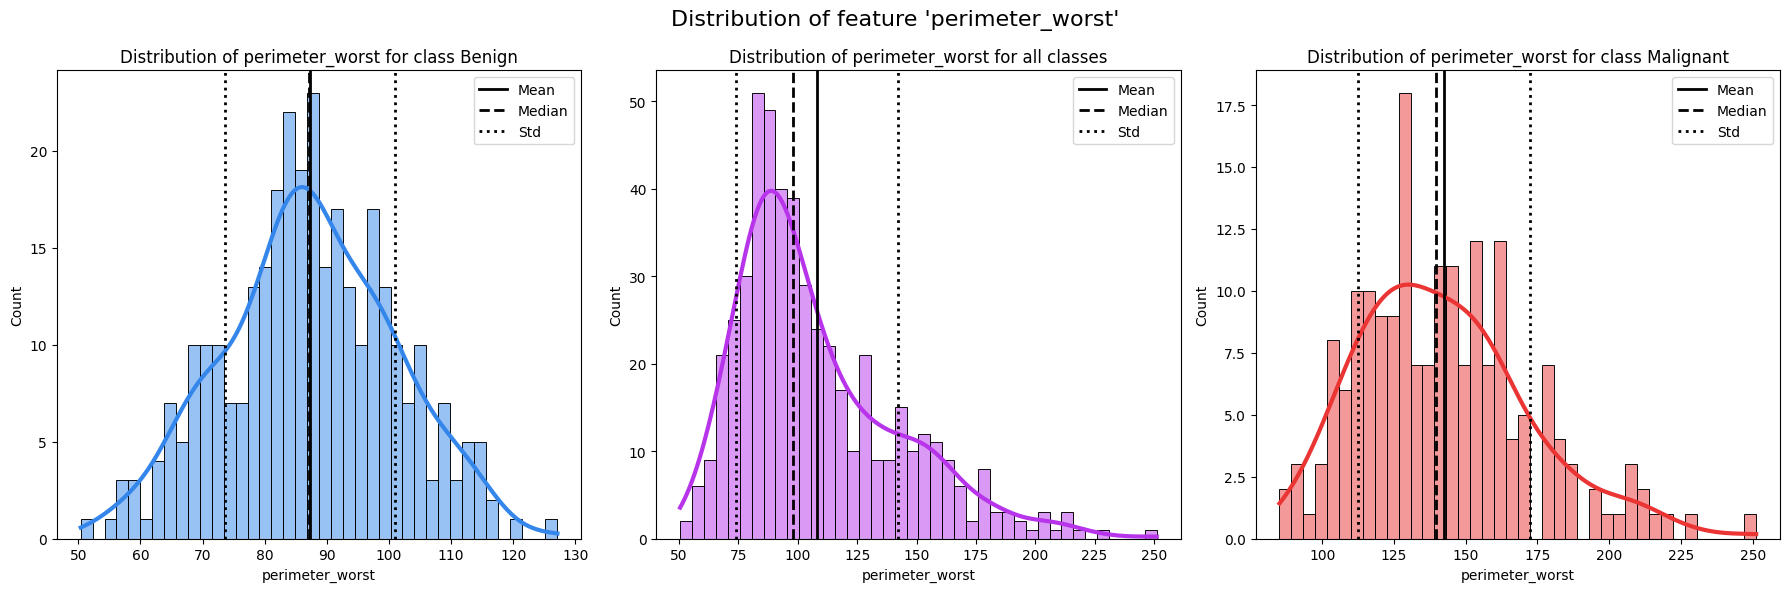
\includegraphics[width=\textwidth]{ims/perimeter_worst.png}
    \caption{Distribution of the \texttt{perimeter\_worst} feature for each
    class (left and right) and the whole dataset (center).}
    \label{fig:perimeter_worst}
\end{figure}

\begin{figure}[H]
    \centering
    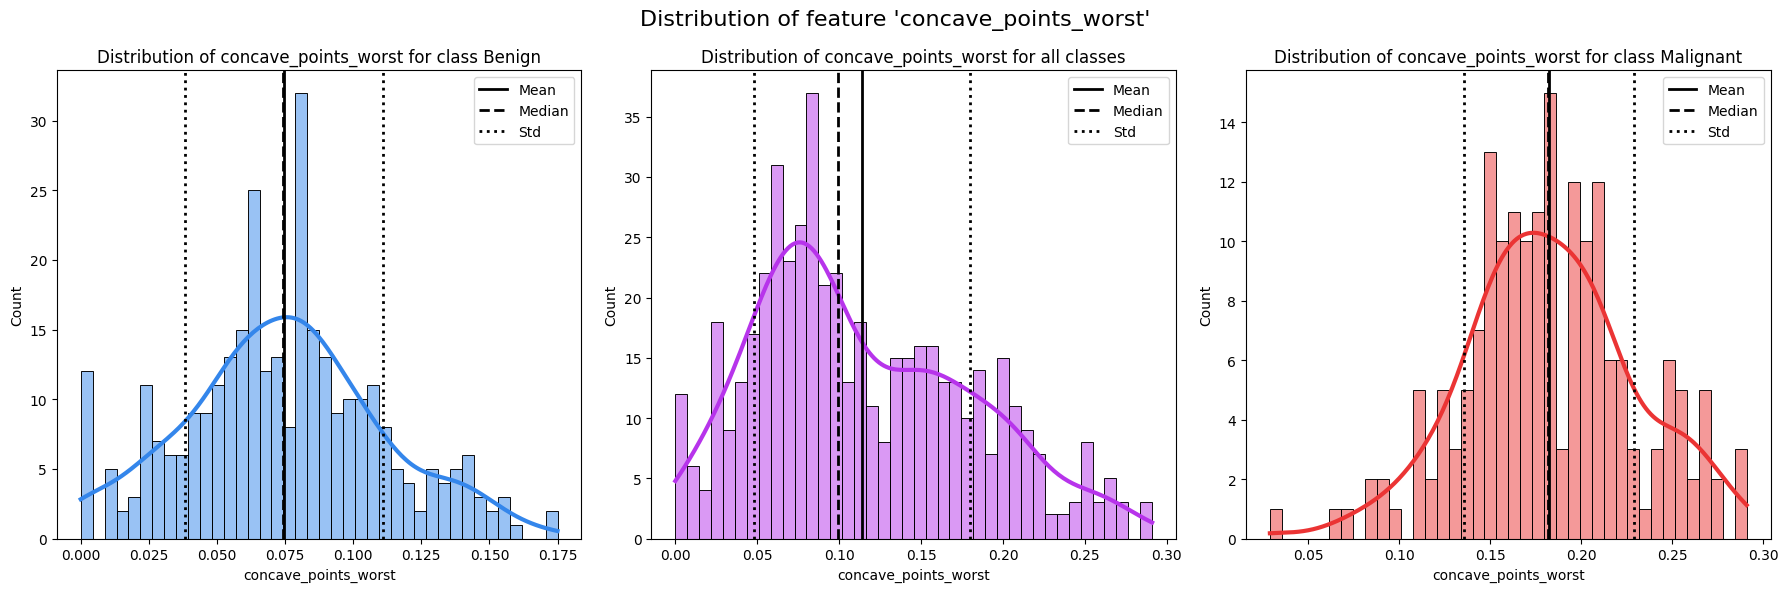
\includegraphics[width=\textwidth]{ims/concave_points_worst.png}
    \caption{Distribution of the \texttt{concave\_point\_worst} feature for each
    class (left and right) and the whole dataset (center).}
    \label{fig:area_worst}
\end{figure}

\begin{figure}[H]
    \centering
    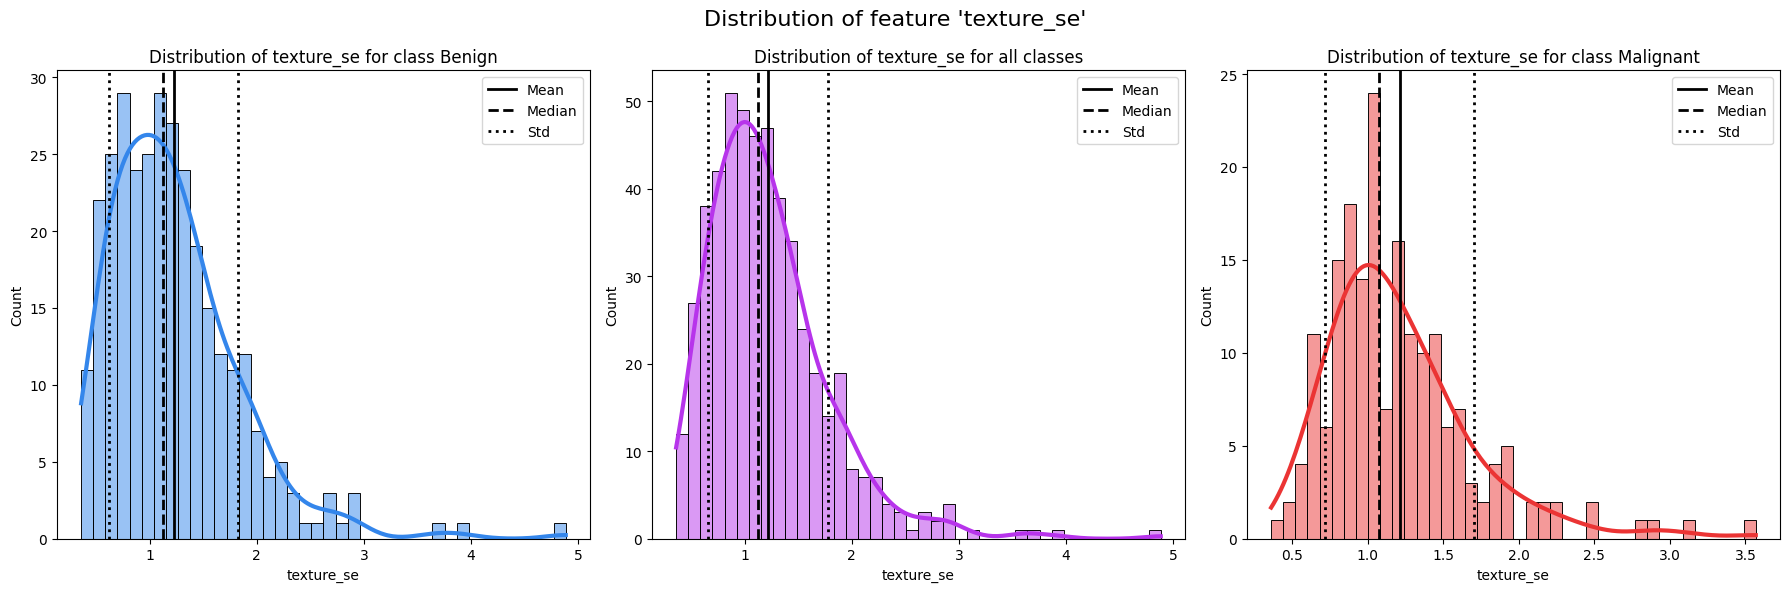
\includegraphics[width=\textwidth]{ims/texture_se.png}
    \caption{Distribution of the \texttt{texture\_se} feature for each class
    (left and right) and the whole dataset (center).}
    \label{fig:concave_points_se}
\end{figure}

In Figure~\ref{fig:perimeter_worst} and Figure~\ref{fig:area_worst}, we can see
that the two classes are well separated, with the malignant class having higher
values for both features. This is not the case in Figure~\ref{%
fig:concave_points_se}; the \texttt{concave\_points\_se} feature has very
similar distributions for both classes.

Next, we can inspect how correlated the features are with the target values by
calculating and plotting the Spearman's $\rho$, Kendall's $\tau$ and the Point
Biserial correlation coefficients. Spearman's $\rho$ and Kendalls's $\tau$ are
useful for measuring non-linear, monotonically increasing relations and the
Point Biserial correlation is specifically designed for binary classification
problems.

In Figure~\ref{fig:corr_coeffs} we can see the absolute values of the
correlation coefficients mentioned above. Eleven values show an absolute
correlation of above 0.6, while only seven being below 0.3, indicating that
the dataset has features that can describe the target value with high accuracy.

\begin{figure}[H]
    \centering
    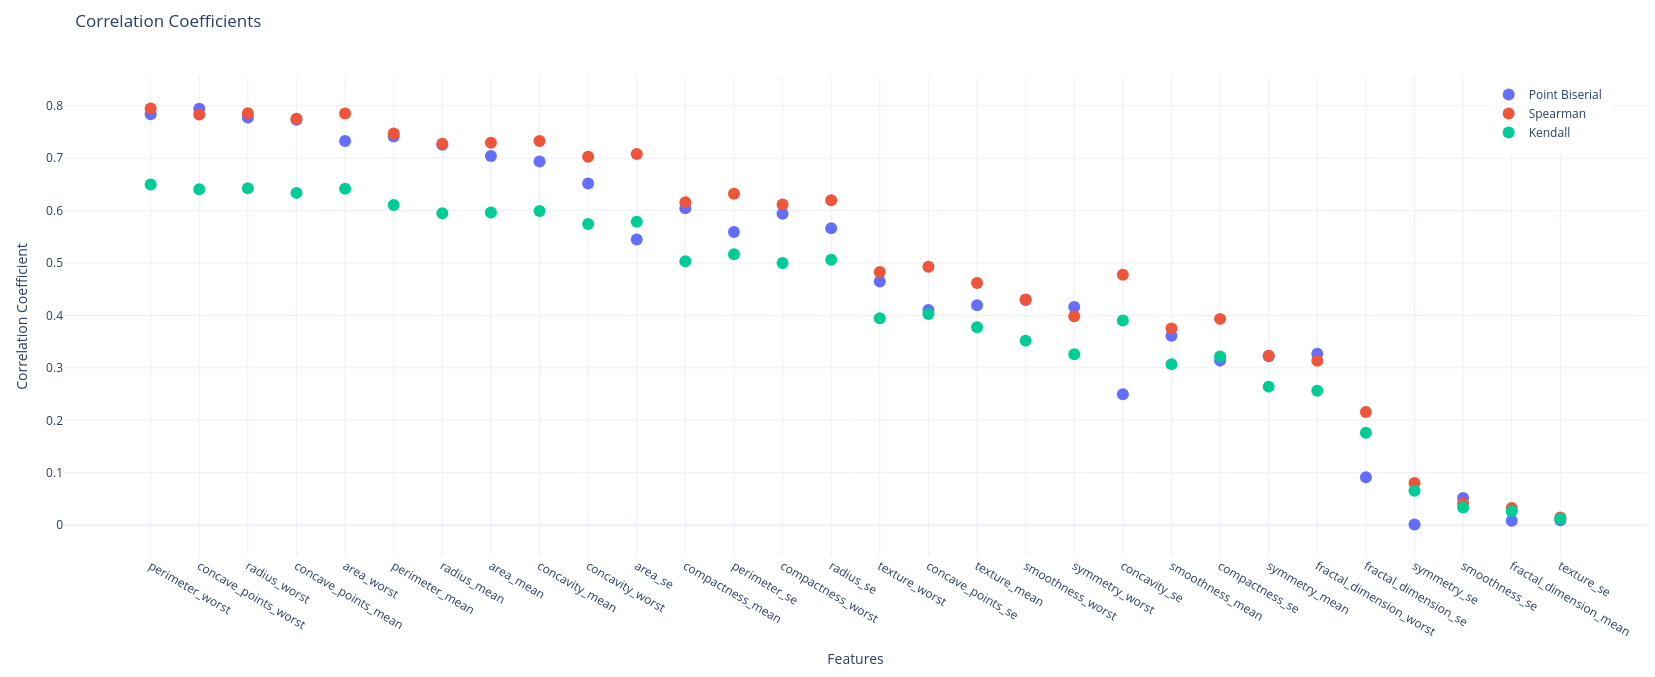
\includegraphics[width=\textwidth]{ims/corr_coeffs.png}
    \caption{Distribution of the Spearman's $\rho$ (red), Kendall's $\tau$
    (green), and Point Biserial (blue) correlation coefficients of all features
    with the target value.}
    \label{fig:corr_coeffs}
\end{figure}

Measuring and plotting the inter-feature correlation can help us find redundant
features. In Figure\ref{fig:corr_coeffs_heatmap} we can see a few examples of
features that seem to carry the same information; these groups of features
appear as spots of high correlation. For example the features regarding the
perimeter and radius show high intra-feature correlation, as well as high
correlation with the features regarding the area. Since I have ordered the
features alphabetically, we expect correlations along the main diagonal to
have high correlation, as they describe the are about features that describe the
same property, and we see that in two main ``blocks''.

\begin{figure}[H]
    \centering
    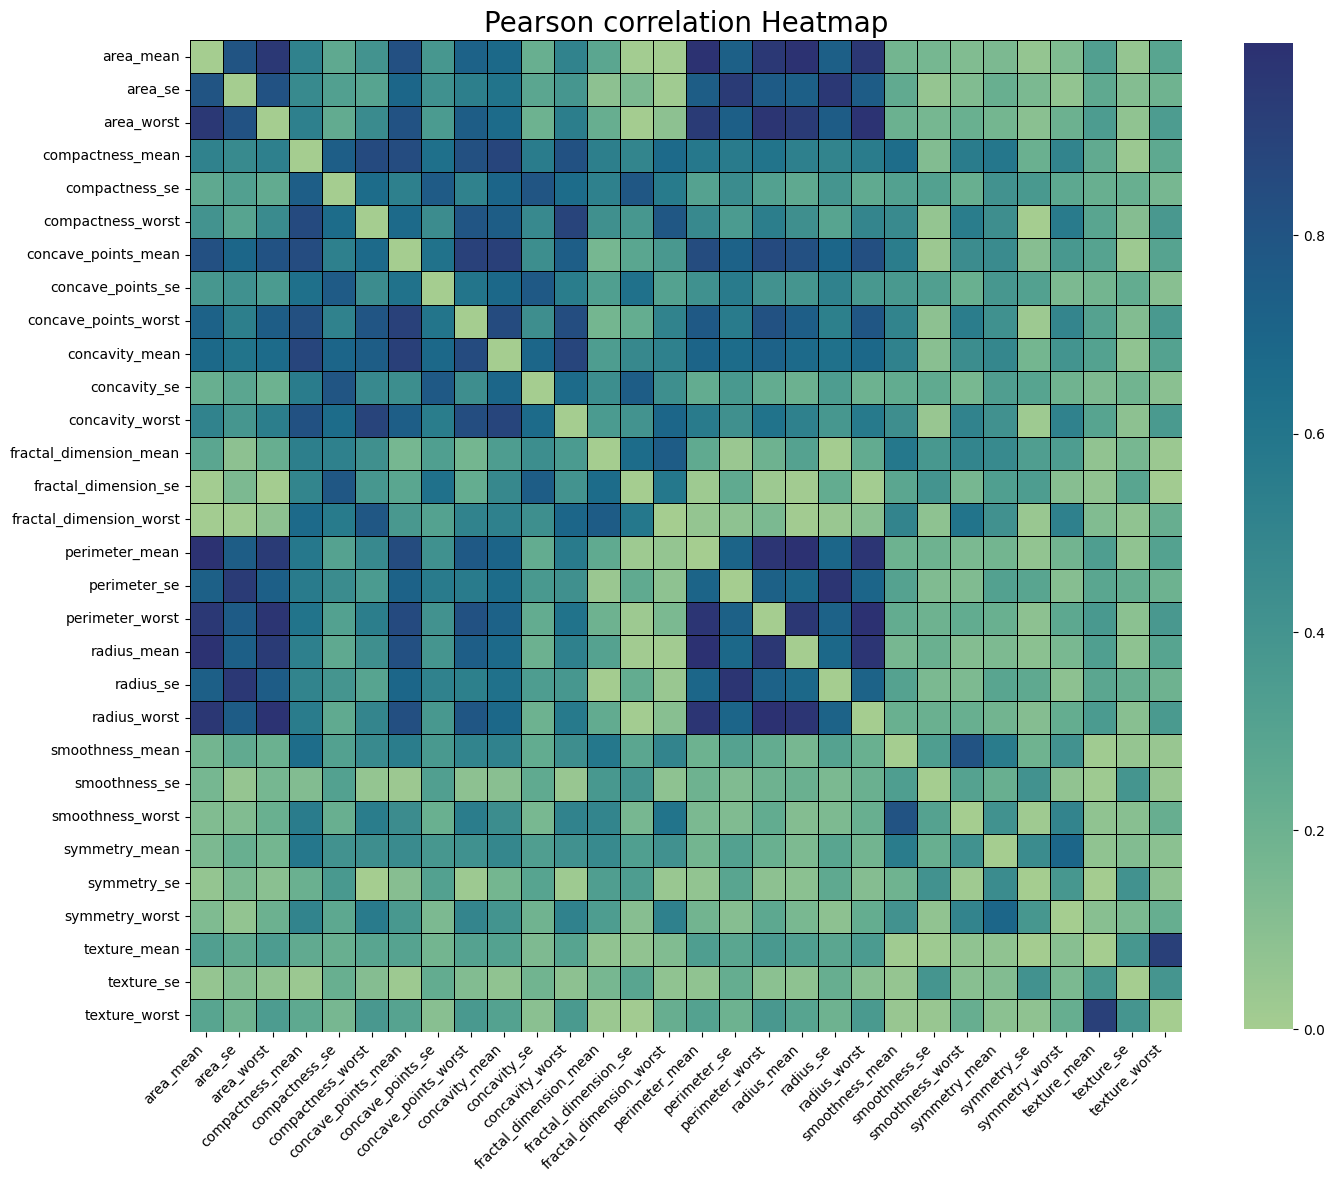
\includegraphics[width=\textwidth]{ims/corr_coeffs_heatmap.png}
    \caption{Distribution of the Spearman's $\rho$ (red), Kendall's $\tau$
    (green), and Point Biserial (blue) correlation coefficients of all features
    with the target value.}
    \label{fig:corr_coeffs_heatmap}
\end{figure}

Overall, the dataset seems to be well separated, with some features being
redundant. I expect that the classifiers will perform well, but I will need to
use feature selection to remove the redundant features and improve the
performance of the classifiers.

Latsly, we can use a dimensionality reduction technique to inspect if the
projections of the data to a subspace show any meaningful separation or if they
form any discernible structure. To that end I used \texttt{PCA}, \texttt{t-SNE},
and \texttt{UMAP} to map thje data points onto a lower dimension and visualize
them. Below, I provide the plots for \texttt{PCA} and \texttt{UMAP}, the
\texttt{t-SNE} results are very similar to the results from \texttt{UAMP} and
they can be found in the \texttt{data\_exploration.ipynb} notebook, I will not
include them here for brevity.

In Figure~\ref{fig:pca} we can see that for the combination of the first and
second principal components, the data set can be somewhat separated, with the
benign class forming a more compact group and the malignant class forming a more
diffuse group, but there is no physical separation between them. A similar
case is true for the combination of the rest of the components. On the other
hand, in Figure~\ref{fig:umap}, we can see that the data points are separated
more clearly, forming a single elongated cluster of points which can be
separated almost exactly at it's center, separating the two classes (in the
cases of the combinations of first and second dimension and first and third).
Furthermore, even from the first dimension, the data seem to from a binomial
distribution, separating the two classes.

\begin{figure}[H]
    \centering
    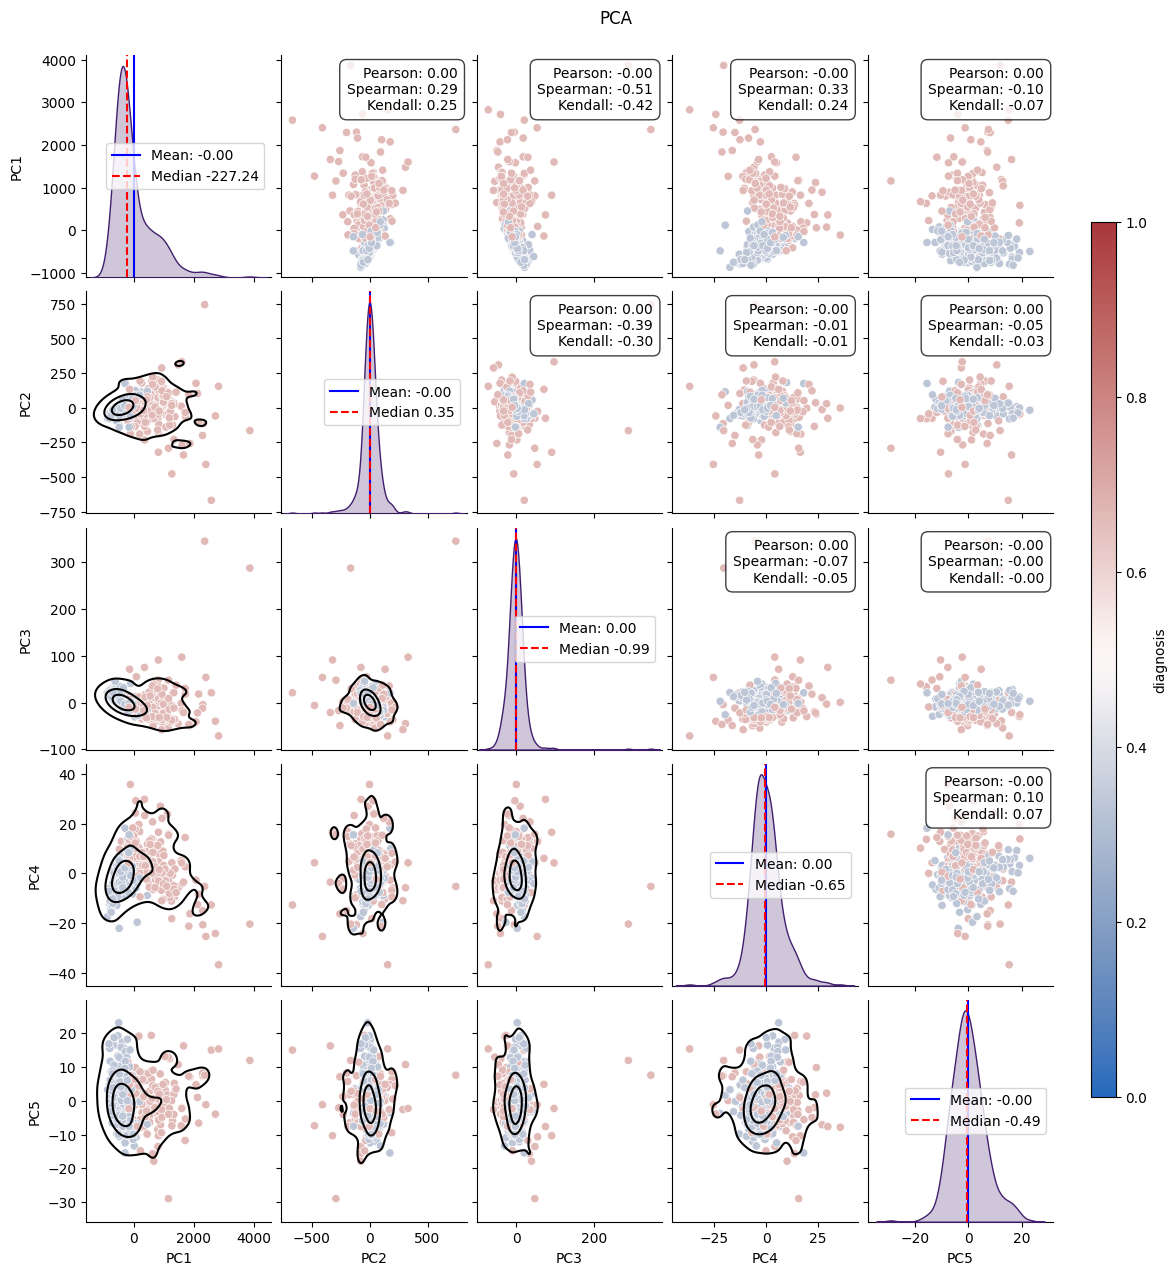
\includegraphics[width=\textwidth]{ims/pca.png}
    \caption{Pairplot of the first 5 prinicpal components after dimensionality
    reduction with \texttt{PCA}. The scatter plots are colored by the target's
    label (blue for benign and red for malignant).}
    \label{fig:pca}
\end{figure}

\begin{figure}[H]
    \centering
    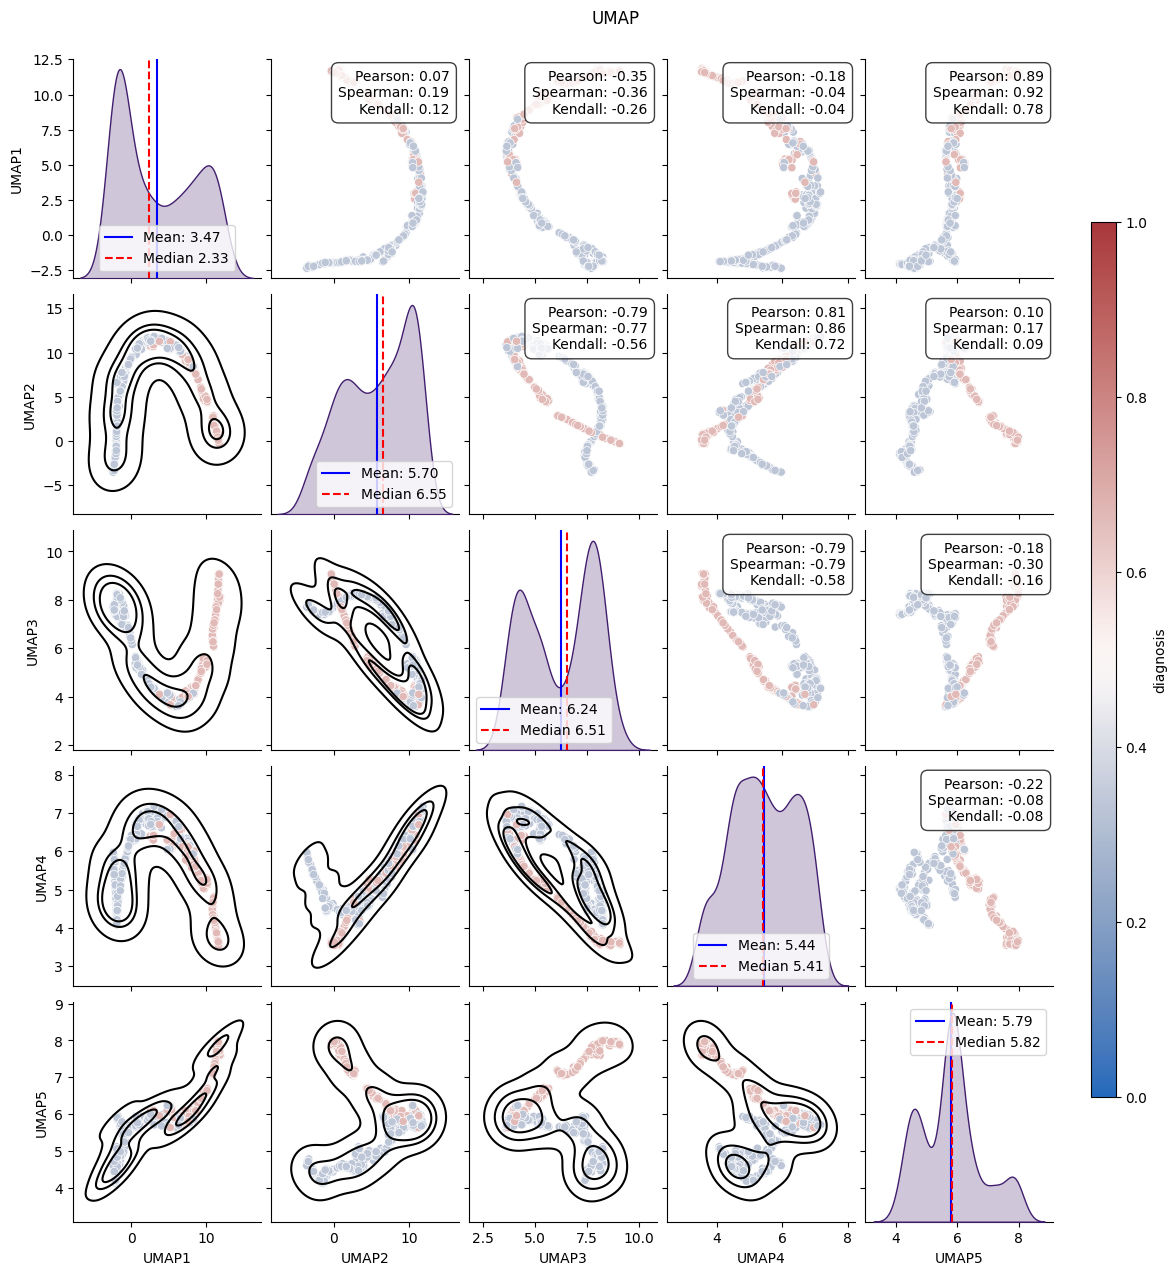
\includegraphics[width=\textwidth]{ims/umap.png}
    \caption{Pairplot of the first 5 embeddings / dimensions after dimensionality
    reduction with \texttt{UMAP}. The scatter plots are colored by the target's
    label (blue for benign and red for malignant).}
    \label{fig:umap}
\end{figure}

With all the above in mind, I decided to set up the \texttt{MrMR} function to
select 10 features, as I have shown that 

%%%%%%%%%%%%%%%%%%%%%%%%%%%%%%%%%%%%%%%%%%%%%%%%%%%%%%%%%%%%%%%%%%%%%%%%%%%%%%%%
%%%%%%%%%%%%%%%%%%%%%%%%%%%%%%%%%%%%%%%%%%%%%%%%%%%%%%%%%%%%%%%%%%%%%%%%%%%%%%%%
% Material and Methods
\section{Material and Methods}

%%%%%%%%%%%%%%%%%%%%%%%%%%%%%%%%%%%%%%%%%%%%%%%%%%%%%%%%%%%%%%%%%%%%%%%%%%%%%%%%
\subsection{Outline}

In essence, a nested cross-validation pipeline consists of two nested loops
(outer and inner loops), encapsulated in a larger loop. In our case, the
encapsulating loops (or rounds) will be set to $R=10$, the outer loops will be
set to $N=5$, and the inner loops to $K=3$.

The job of the outer fold is to split the data set and perform cross-validation,
with the inner folds performing hyperparameter tuning with yet another
cross-validation. The job of the enclosing rounds is to change the random number
generator seeds, to get $R$ different results, leading to better generalization
ability of the model. A schematic of nested cross-validation is provided below
(Figure\ref{fig:ncv_scheme}).

\begin{figure}[H]
    \centering
    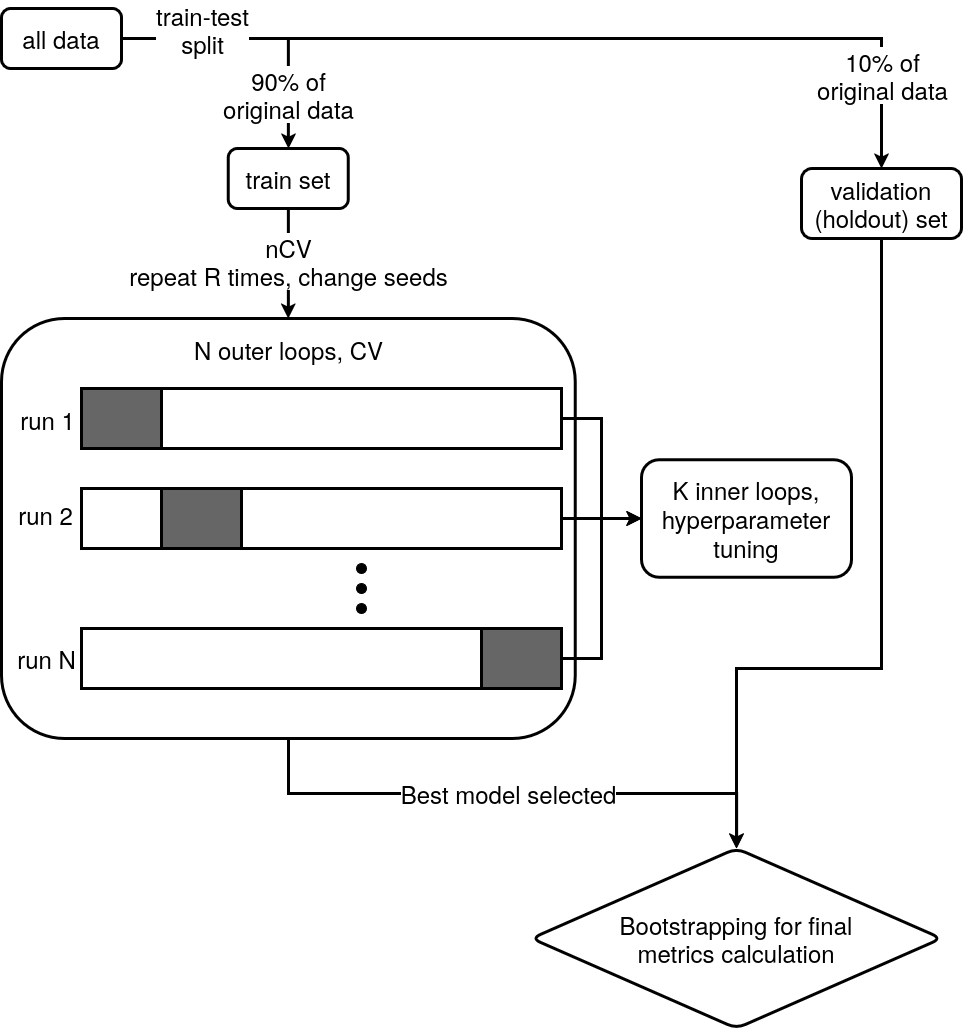
\includegraphics[width=0.9\textwidth]{ims/nCV.drawio.png}
    \caption{Nested cross-validation scheme. A holdout set is first taken from
    the dataset, here set to $10\%$. Then, $R$ times, the model is trained
    using cross-validation ($N$ splits), with an inner loop of hyperparameter
    tuning, which is also done using cross-validation ($K$ splits). All
    training results are aggregated and the best set of hyperparameters
    is selected. After all models are trained, the best one can be tested
    against the unseen data (holdout set); here metric statistics are
    calculated using resampling with bootstrapping.}
    \label{fig:ncv_scheme}
\end{figure}

The implementation of a nested cross-validation is easy, but it needs extra
care to avoid data leakage. The data must be scaled inside the inner loop, after
their final split, otherwise the training set will carry some information of the
test set (and as always the scaler must be fitted only on the test set). I
decided to perform feature selection using the whole training set, ignoring the
fact that it might ``leak'' some information to the rest of the pipeline, as I
believe it will be minimal.

%%%%%%%%%%%%%%%%%%%%%%%%%%%%%%%%%%%%%%%%%%%%%%%%%%%%%%%%%%%%%%%%%%%%%%%%%%%%%%%%
%%%%%%%%%%%%%%%%%%%%%%%%%%%%%%%%%%%%%%%%%%%%%%%%%%%%%%%%%%%%%%%%%%%%%%%%%%%%%%%%
% Results and Discussion
\section{Results and Discussion}




\end{document}